\documentclass[final]{beamer}
\usepackage[utf8]{inputenc}
\usepackage[spanish]{babel}
\usepackage{amsmath,amssymb,amsthm,amsfonts}
\usepackage{graphicx}
\usepackage{tikz}
\usepackage{animate}
\usepackage{multimedia}
%%%%%%%%%%%%%%%%%%%%%%
\title{Modelos multiagentes}
\author{Augusto Cabrera Becerril}
\date{\today}
\institute{Facultad de Ciencias UNAM}

%%%%%%%%%%%%%%%%%%%%%%


%%%%%%%%%%%%%%%%%%%%%%%%

\mode<presentation>
\usetheme{Berlin}
\usecolortheme{wolverine}
%%%%%%%%%%%%%%%%%%%%%%%

\begin{document}
\begin{frame}
\maketitle
\end{frame}

\begin{frame}{Sistemas Complejos}
\section{Primera}
    \begin{abstract}
    En esta platica  hablaremos de modelos directos de sistemas complejos adaptativos   
    \end{abstract}
    
\end{frame}

\begin{frame}{Imágenes}
\section{segunda}
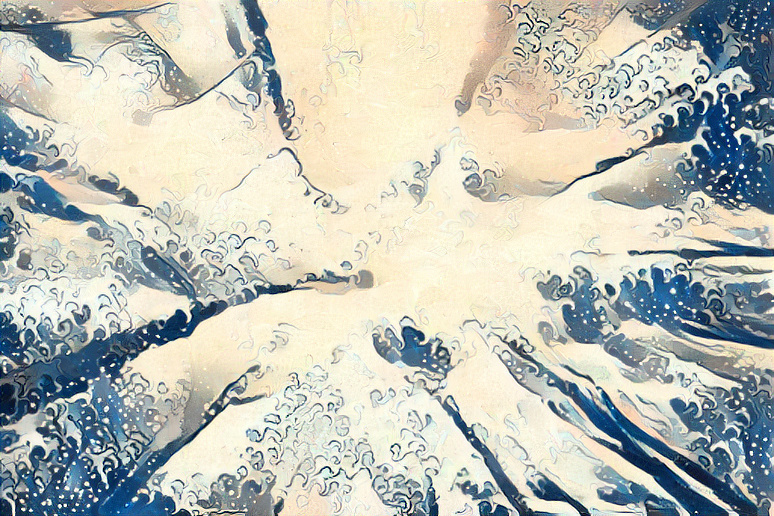
\includegraphics[width=\textwidth]{imagen1.jpg}
\end{frame}

\begin{frame}{Modelos Basados en Agentes}
\section{Tercera}
\pause
    \begin{enumerate}
        \item Agentes
        \pause
        \item Mundo
        \pause
        \item Reglas de interacción
    \end{enumerate}
\end{frame}

\begin{frame}{Animación con png}
    \animategraphics[autoplay,loop,scale=0.3]{10}{ATT-}{0}{26}
\end{frame}

\begin{frame}{Texto animado}
    En una galaxia muy lejana \pause
    alguien aprende a usar Beamer \pause
    y usa animaciones para llamar la atención
\end{frame}


\end{document}
